% ----------------------------------------------------------
\chapter{Introdução}\label{cap:introducao}
% ----------------------------------------------------------

Estamos vivenciando um crescimento exponencial no número de dispositivos conectados à internet, impulsionado principalmente pela expansão da Internet das Coisas (IoT). Essa categoria abrange uma ampla gama de equipamentos, como smartphones, relógios inteligentes, sensores ambientais, eletrodomésticos inteligentes e veículos autônomos, entre outros. Esses dispositivos diferem significativamente entre si em termos de capacidade computacional, armazenamento local, autonomia energética e protocolos de comunicação utilizados, o que introduz desafios consideráveis de interoperabilidade e gerenciamento em larga escala.

Paralelamente, cresce a exigência por processamento de dados em tempo quase real, especialmente em aplicações de missão crítica. Veículos autônomos, por exemplo, precisam realizar inferências e tomar decisões instantâneas com base em grandes volumes de dados sensoriais \cite{markakis2017}. Da mesma forma, em cenários de saúde digital, dispositivos vestíveis como \textit{smartwatches} monitoram sinais vitais continuamente e podem enviar alertas automáticos a instituições médicas, possibilitando respostas emergenciais, como o envio imediato de ambulâncias em situações críticas \cite{cassel2024}.

Diante desse cenário, a arquitetura de computação em névoa (\textit{fog computing}) surgiu como uma solução eficaz para suprir a necessidade de processamento e armazenamento mais próximos da borda da rede. Essa abordagem reduz a latência e melhora a eficiência do sistema, sendo especialmente relevante em aplicações que exigem respostas rápidas e precisas. A computação em névoa ainda pode atuar como intermediária entre os dispositivos e a nuvem, realizando um pré-processamento local dos dados antes de enviá-los para a nuvem, o que facilita a integração, reduz o tráfego e diminui a carga sobre os servidores centrais.

Na Figura~\ref{fig:arquitetura_basica}, temos ilustrado uma arquitetura básica de névoa, os dispositivos enviam dados para os equipamentos da camada de névoa, onde ocorre o processamento local. Os dados processados podem então ser devolvidos para os dispositivos ou encaminhados à nuvem, dependendo do contexto da aplicação.

\begin{figure}[htb]
	\caption{\label{fig:arquitetura_basica}Arquitetura básica de comunicação na computação em névoa.}
	\begin{center}
		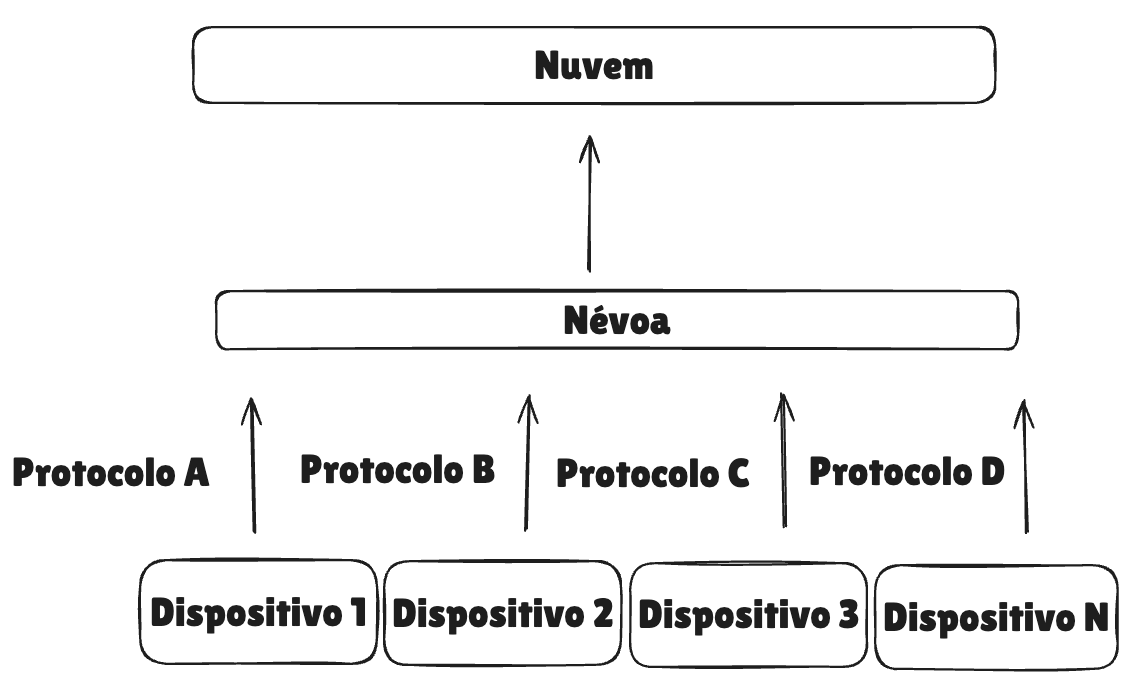
\includegraphics[width=0.7\linewidth]{images/arquitetura_basica.png}
	\end{center}
	\fonte{Do autor.}
\end{figure}

No entanto, a diversidade de dispositivos e protocolos de comunicação ainda representa um obstáculo à interoperabilidade plena. A ausência de um padrão universalmente aceito dificulta a comunicação eficiente entre equipamentos heterogêneos.

Para abordar esses desafios, este trabalho propõe uma arquitetura de névoa modular com suporte à comunicação entre diferentes névoas, a qual é composta por três camadas principais, descritas a seguir:

\begin{itemize}
    \item \textbf{Nó de Névoa Primário:} responsável por atuar como ponto de entrada da arquitetura de névoa. Ele realiza a conversão de protocolos de comunicação, o balanceamento de carga entre os demais nós de névoa e outros nós primários, além de localizar e coordenar os nós de névoa disponíveis.

    \item \textbf{Nó de Névoa:} recebe os dados encaminhados pelo nó primário, realiza o pré-processamento local conforme a lógica da aplicação, e transmite os resultados ao nó agregador.

    \item \textbf{Nó Agregador:} responsável por consolidar os dados processados pelos diversos nós de névoa em um único arquivo ou estrutura de dados, facilitando sua transmissão para a nuvem.
\end{itemize}

% ----------------------------------------------------------
\section{Objetivos}
% ----------------------------------------------------------

Nas seções abaixo estão descritos o objetivo geral e os objetivos 
específicos.

% ----------------------------------------------------------
\subsection{Objetivo Geral}
% ----------------------------------------------------------

Desenvolver uma arquitetura modular de computação em névoa voltada à comunicação entre diferentes névoas, com foco na integração de novos dispositivos, e na facilitação da interoperabilidade entre protocolos distintos, considerando aplicações cujos requisitos possam ser contemplados por essa abordagem.

% ----------------------------------------------------------
\subsection{Objetivos Específicos}
% ----------------------------------------------------------

Para atender ao objetivo geral descrito nesta seção, apresentam-se os seguintes objetivos específicos:

\begin{itemize}
  \item Desenvolver uma arquitetura modular em camadas para a computação em névoa, definindo as funções e responsabilidades de cada camada, com foco na integração de novos dispositivos.
  
  \item Projetar e implementar um sistema de comunicação entre névoas, visando facilitar a interoperabilidade e reduzir a latência entre dispositivos que utilizam diferentes padrões e tecnologias, atendendo a aplicações cujos requisitos sejam compatíveis com a arquitetura.

  \item Desenvolver e integrar mecanismos de conversão de protocolos, permitindo a comunicação entre dispositivos com diferentes padrões e tecnologias.

  \item Avaliar a eficácia da arquitetura modular proposta por meio da medição de tempo de resposta, latência e quantidade de pacotes com e sem falhas, em simulações que reproduzam requisitos específicos das aplicações.

  \item Documentar os resultados obtidos e propor diretrizes, fornecendo orientações e melhores práticas para futuras implementações e pesquisas que atendam a requisitos similares.
\end{itemize}
